% Porfavor no cambiar el formato, este es el exigido por el Encuentro Chileno de la Computacion.
% Mantenerlo así hasta el 15/07/2008.
% Idioma: español, inglés o portugués.
% Tamaño 8 1/2" x 11" (carta, letter USA), máximo 10 páginas, incluyendo resumen no superior a
% 130 palabras.
% Márgenes: superior 3,5 cm, inferior 2 cm, derecho e izquierdo: 2,5 cm.
% Formato: Texto justificado a la derecha e izquierda, páginas no numeradas.
% Tipo de letra: Times 10 para el texto y 12 para títulos y apartados.
% La primera página debe contener: El título del trabajo, nombre completo de autores, afiliación y
% direcciones, así como el resumen del trabajo y palabras claves para su clasificación sobre la base de
% los temas propuestos en este llamado.

\documentclass[letterpaper,12pt]{article}
\usepackage{graphicx}
\usepackage{url}
\usepackage[utf8]{inputenc}
\usepackage{enumerate}
\usepackage{listings}
\usepackage{colortbl} 

%opening
\title{ Autenticación JAAS para máquinas JBoss}

\author{
Esteban F. Bombal,
Rodrigo G. Fernández,
Cristián D. Maureira,\\
Ignacio J. Villacura,
Gabriel A. Zamora
}

\begin{document}
\bibliographystyle{plain}
\pagestyle{empty}

\maketitle\thispagestyle{empty}

\begin{abstract}
El presente documento aborda lo que es el proyecto de Control de Acceso Lógico para el
servidor de aplicaciones JBoss~\cite{JBOSS}. Nuestro grupo de trabajo se enfoca en la implementación de 
un framework de seguridad llamado JAAS~\cite{JAAS}, basado en la tecnología JAVA~\cite{JAVA}, además de establecer una conexión
a servicios de directorios mediante LDAP~\cite{OpenLDAP} para la conexión a una máquina JBoss.

\end{abstract}

Palabras Clave: Java, Servidores, Autentificación, JBoss, JAAS, LDAP

\newpage
\section{Introducción}
\label{sec:introduccion}
%1-introduccion. Explicar el contexto, problema abordado y los objetivos del trabajo. Definir cómo está organizado el informe.

\subsection{Contexto}
El Control de Acceso Lógico a aplicaciones y sistemas es el primer obstáculo a
superar por un “atacante” para el acceso no autorizado a un equipo y a los
datos que contiene. La utilización de métodos de seguridad combinados como la
biometría permite reducir la probabilidad de éxito en los intentos de acceso
por personal no autorizado.

Los Controles de Acceso lógico son de vital importancia ya que permiten
proteger los recursos de los equipos. Esto se acrecienta cuando estos recursos
almacenan información confidencial, documentos clasificados, bases de datos
internas del ejército y/o Ministerio de Defensa de un país.

Este documento es una base para aplicar Control de Acceso Lógico en una máquina
JBoss, para sus aplicaciones pertinentes, específicamente utilizando la API \emph{JAAS}.

\emph{JAAS} son las siglas de \emph{Java Authentication and Authorization}. Se
trata de una especificación integrada en la máquina virtual Java a partir de
la versión 1.4 y cuya finalidad es la de definir un estándar para los procesos
de autentificación y autorización.

Es decir ambos procesos, autentificación y autorización están directamente
relacionados con la seguridad de aplicaciones.

Para contextualizar de una mejor manera definiremos los conceptos de \emph{autentificación} y \emph{autorización}.

La \emph{autentificación} es el proceso por el cual un usuario o servicio tiene que
autentificarse para poder acceder a ciertos servicios que ofrece el sistema.

Existen distintas categorías de autentificación:
\begin{itemize}
	\item \textbf{¿Qué sabes?}: Información que el usuario conoce. Ej: Contraseñas, respuestas a preguntas como: "Nombre de tu mascota".
	\item \textbf{¿Qué tienes?}: Elementos físicos que el usuario posee. Ej: Tarjetas bancarias.
	\item \textbf{¿Quién eres?}: Técnicas biométricas como lectura de retina o huellas dactilares.
\end{itemize}

\newpage

La \emph{autorización} es el proceso por el cual se controlan las acciones que tiene
un usuario o servicio normalmente ya autenticado puede realizar, para ello se le
conceden o deniegan permisos.

Categorías de autorización:
\begin{itemize}
    \item \textbf{Autorización declarativa}: En este tipo de autorización los privilegios son gestionados un administrador independientemente de manera externa al código de la aplicación
    \item \textbf{Autorización programática}: En este tipo de autorización las decisiones de autorización se realizan desde el código fuente de la aplicación.
\end{itemize}

\subsection{Objetivos}

Los objetivos específicos planteados en este informe, para la configuración y funcionamiento de la aplicación JAAS sobre máquina JBoss son los siguientes:

\begin{itemize}
	\item Instalación de API JAAS
	\item Integración de LDAP en JBoss usando JAAS
	\item Integración de JAAS en Tomcat
	\item Implementación de Single Sign-On
\end{itemize}


\section{Fundamentos Técnicos}
\label{sec:fundamentosTecnicos}
%2-fundamentosTecnicos. Conceptos fundamentales y trabajos relacionados sobre los que se sustenta el proyecto desarrollado. Referenciar trabajos relevantes.

\subsection{Conceptos Fundamentales}
\begin{description}
	\item[JAAS:]
Java Authentication and Authorization Service, es una Interfaz de Programación de Aplicaciones que permite a las
aplicaciones Java acceder a servicios de control de autenticación y acceso.
	\item[JBoss:]
JBoss es un servidor de aplicaciones J2EE de código abierto implementado en
Java puro. Al estar basado en Java, JBoss puede ser utilizado en cualquier
sistema operativo que lo soporte.

JBoss implementa todo el paquete de servicios de J2EE.

%El servidor de aplicaciones JBoss cuenta con utiliza dentro de el las siguientes herramientas:
%\begin{itemize}
%	\item JBoss AOP
%	\item Hibernate
%	\item JBoss Cache
%	\item JBoss IDE
%	\item JBoss jBPM
%	\item JBoss Portal
%	\item JGroups
%	\item Tomcat
%	\item JBoss Mail Server
%	\item JBoss MQ
%	\item JBoss Messaging
%	\item JBoss Forum
%\end{itemize}

	\item[SSO:]
Single sign-on (SSO) es un procedimiento de autenticación que habilita al
usuario para acceder a varios sistemas con una sola instancia de
identificación.

Hay cinco tipos principales de SSO, también se les llama reduced sign on
systems (en inglés, sistemas de autenticación reducida).
\begin{itemize}
	\item Enterprise single sign-on (E-SSO)
	\item Web single sign-on (Web-SSO),
	\item Kerberos
	\item Identidad Federada
	\item OpenID
\end{itemize}
\item[Servlet:] Los servlets son objetos que corren dentro del contexto de un
contenedor de servlets (ej: Tomcat) y extienden su funcionalidad. También
podrían correr dentro de un servidor de aplicaciones, que, además de
contenedor para servlet, tendrá contenedor para objetos más avanzados, como
son los EJB (Tomcat sólo es un contenedor de servlets).

\end{description}

\subsection{Trabajos Relacionados}

A continuación algunos trabajos relacionados con el presente estudio
realizado:

\begin{itemize}
	\item User authentication and authorization in the JavaTM platform.~\cite{paper4}
	\item An operational semantics of Java 2 access control.~\cite{paper1}
	\item A Comparative Study of Access Control Languages.~\cite{paper2}
	\item Automated generation of enforcement mechanisms for semantically-rich security policies in Java-based multi-agent systems.~\cite{paper3}
\end{itemize}


\section{Análisis}
\label{sec:analisis}
%3-analisis. Identificación, evaluación y selección de alternativas para el proyecto
Para cada objetivo planteado al comienzo de este reporte se analizaron las
alternativas existentes actualmente y según cada caso se plantea la selección
de las mas adecuadas:
\begin{itemize}
	\item \textbf{Instalación API JAAS}: Para este primer paso la única
manera de proceder es seguir los pasos descritos más adelante para contar con
la API \emph{JAAS} funcional.
	\item \textbf{Integración de LDAP en JBoss usando JAAS}: Tomando en
consideración que \emph{JBoss} usa el módulo LoginLdapModule para conectarse
con \emph{LDAP} es necesario configurar este módulo para usar la autenticación y la autorización mediante \emph{JAAS}
	\item \textbf{Integración de JAAS en Tomcat}: Aunque es posible utilizar
JAAS en Tomcat como un mecanismo de autenticación (JAASRealm), la flexibilidad
del marco de JAAS se pierde una vez que el usuario se autentica. Esto es porque
los principios usados para designar al "usuario" y "rol", ya no están disponibles
en el contexto de seguridad en el que se ejecuta la webapp. El resultado de la
autenticación sólo está disponible a través de request.getRemoteUser() y
request.isUserInRole().

Esto reduce el marco de JAAS para fines de autorización a un simple usuario/sistema
de roles, que pierde su conexión con la política de seguridad de Java. 

Es por esto que la solución planteada en este reporte técnico es ajustar la ejecución de los servlets en la implementación de JAAS, de manera que nos permita reforzar el control de acceso con una simple llamada en nuestro código.
\end{itemize}


\section{Diseño e Implementación}
\label{sec:disenoImplementacion}
%4-disenoImplementación. Aspectos específicos sobre diseño e implementación del proyecto.

\subsection{Diseño}

En este proyecto, lo que se desea desarrollar, es permitir el acceso a diferentes tipos de sistemas a través del servicio de autenticación JAAS, mediante el uso de Single Sign On, sobre la plataforma Jboss.

Primeramente se desea que el futuro usuario, al momento de comenzar la utilización del sistema, se le provea un sistema en el cual pueda ingresar su usuario y correspondiente contraseña. Para establecer si el usuario que trata de ingresar al sistema, posee los respectivos permisos para ello, se hace uso de un sistema de directorio del tipo LDAP, el cual posee una estructura jerárquica con los respectivos usuarios permitidos. Una vez que se valida la autenticación, dependiendo del usuario que haya ingresado, se le asigna un ``rol'', el cual dependiendo de la configuración de JBoss, le dará los permisos de acceder a los diferentes servicios web disponibles para él. Además al disponer habilitado el sistema ``Single Sign On'', una vez que el usuario ha ingresado por primera vez al sistema, puede acceder a los diferentes servicios provistos para su rol, sin la necesidad de ingresar sus datos para la autenticación nuevamente.

He acá un diagrama explicando lo anterior:\\

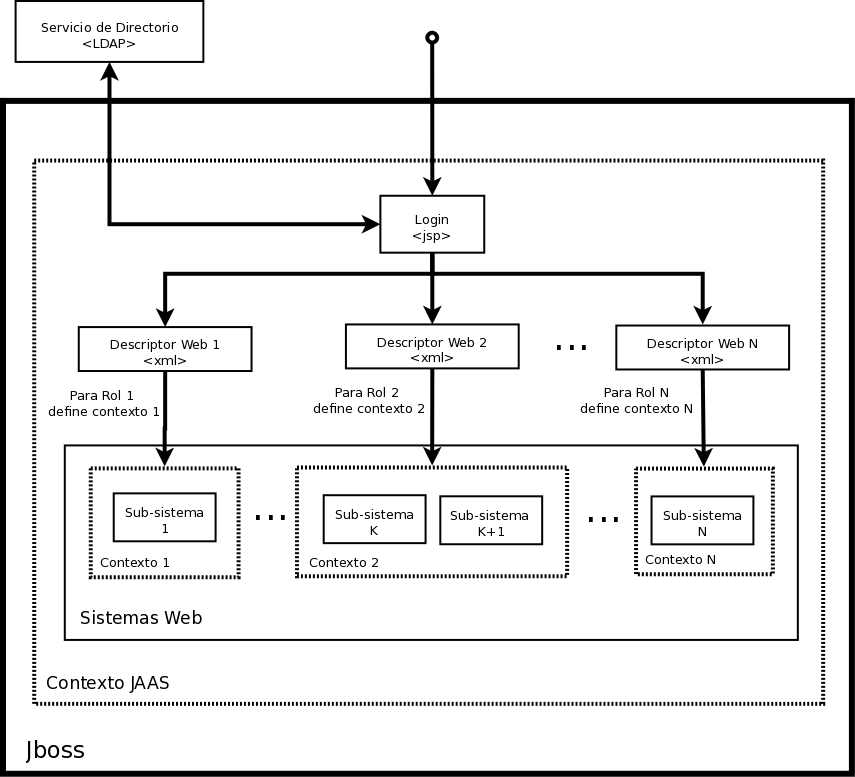
\includegraphics[scale=0.35]{img/diseno}

\subsection{Implementación}
\lstset{basicstyle=\tiny, breaklines=true, numbers=left,
frame=shadowbox, rulesepcolor=\color{black}}

	\subsubsection{Instalación de base de datos LDAP}
	\begin{enumerate}
		\item Bajar e instalar OpenLDAP.
		\item Configurar slapd.conf (hay que especificar el suffix, rootdn (usuario al
cual JBoss se conectará), rootpw, y opcionalmente el directorio.
		\item  Necesitamos tener los necesarios usuarios y grupos en LDAP que serán
utilizados en JBoss. Esto debe configurarse en el servidor LDAP previamente.
	\end{enumerate}

	\subsubsection{Implementación del SSO en JBoss}
	\begin{enumerate}
		\item Para activar SSO, simplemente activamos la opción en el archivo
de configuración de TomCat: JBOSS\_HOME/server/tu\_configuracion/deploy/jboss-web.deployer/server.xml.

	\end{enumerate}
	\subsubsection{Integración de LDAP utilizando JAAS en servidores web JBoss}
	\begin{enumerate}
			\item JBoss usa el LoginLdapModule para conectarse con LDAP.
			Configuramos la application-policy en el login-config.xml que puede ser encontrado en JBOSS\_HOME/server/default.conf. Esto permitirá a JBoss conectarse con el servidor LDAP y le dirá la estructura que debe tener, como su usuario, password y los roles que encontrará.
			\item Después de esto solo nos queda conectarnos a través de una
aplicación JAAS. En nuestro caso utilizamos un Servlet que probara la
conexión realizando ciertas consultas a la base de datos.
	\end{enumerate}
%	\item Integración con otros proyectos
%	\begin{enumerate}
%		\item 
%
%	\end{enumerate}


\section{Resultados}
\label{sec:resultados}
%5-resultados. Pruebas, mediciones, resultados y conclusiones

\begin{enumerate}

\item \textbf{Pruebas:} La mayor parte de las pruebas se hicieron cuando se tuvo configurado el
servidor \emph{JBoss} con \emph{JAAS} y \emph{SSO}. La única forma de saber si la configuración fue la correcta, es
con un servlet en el servidor Tomcat que intentase autentificar con usuario y contraseña al
servidor \emph{JBoss}. Esta es la única forma de ver en forma tangible si la configuración tiene todo lo necesario.

\item \textbf{Resultados:} Los resultados obtenidos son varios. En primer lugar fue factible
habilitar autentificación vía \emph{JAAS} en un servidor \emph{JBoss}. Por otro lado se logro que se pudiese
autentificar contra \emph{LDAP} al igual que utilizara el \emph{SSO} para sesiones independientes. Lo único
que no se llevo a cabo fue la integración con los demás grupos, todos los resultados obtenidos
fue en un servidor de pruebas propio.

\item \textbf{Conclusiones:} Si bien no se logro la integración con los demás grupos se usaron
todos los servicios que se requerían, ya sea \emph{LDAP}, \emph{Tomcat} y \emph{JBoss}. Por otro la configuración
de \emph{JAAS} y \emph{SSO} fue bastante simple en el servidor \emph{JBoss}, no así la implementación de un servlet
que integra todo lo visto para poder ver tangiblemente. Este punto fue el mas difícil ya que se
tuvo que programar. 
Finalmente, podemos darnos cuenta que \emph{JAAS} es una herramienta bastante útil en cuanto a
\emph{Control de Acceso Lógico}, para poder restringir el uso de aplicaciones en un servidor determinado;
y si se une con el método \emph{Single Sign-On}, se convierte en una opción totalmente viable para la autenticación
y autorización de usuarios.
\end{enumerate}


\bibliography{reporteTecnico,url}
\vfill \hfill EBG/RFG/CMF/IVD/GZN/DI/UTFSM/2009
\end{document}

%%% Local Variables: 
%%% mode: latex
%%% TeX-master: t
%%% End: 
